\chapter{Einleitung}

\begin{figure}[H]
	\centering
	\begin{minipage}{.5\textwidth}
		\centering
		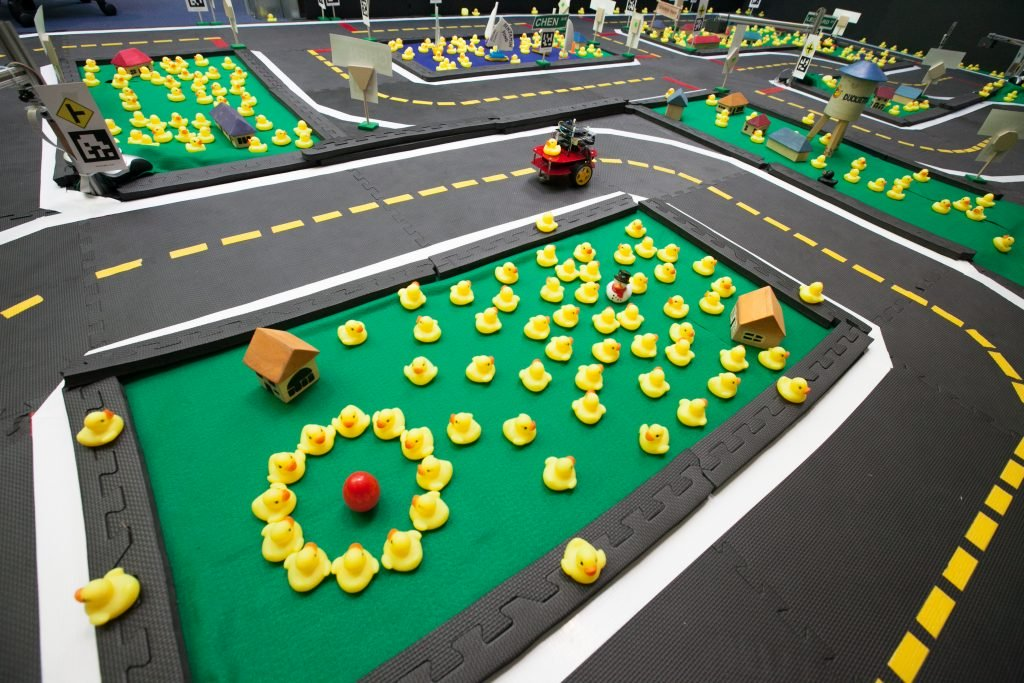
\includegraphics[width=0.95\textwidth]{kapitel1/images/duckietown.png}
		\quelle\url{https://www.duckietown.org/wp-content/uploads/2018/05/duckietown_nice-1024x683.jpg}
		\label{fig:duckietown}
	\end{minipage}%
	\begin{minipage}{.5\textwidth}
		\centering
		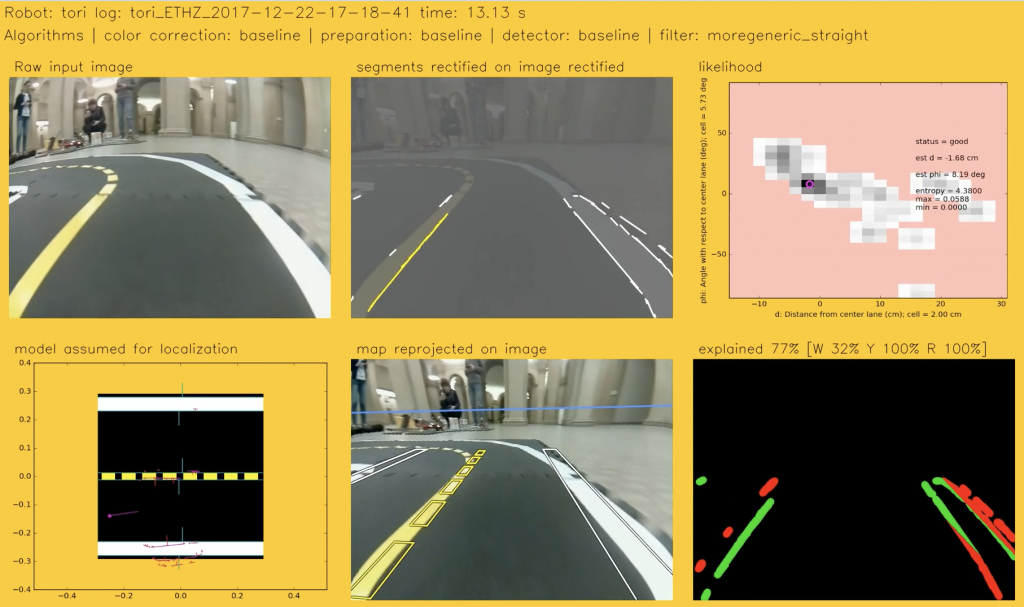
\includegraphics[width=1.072\textwidth]{kapitel1/images/duckietown2.png}
		\quelle\url{https://www.duckietown.org/wp-content/uploads/2018/06/data-from-img-CameraDataProcessed-fc6fd822-1024x607.png}
		\label{fig:duckietown2}
	\end{minipage}
	\caption{Duckietown}
\end{figure}

Das Duckietown-Projekt wurde 2016 am \acf{mit} konzipiert. Das Ziel war es, eine Plattform zu
entwickeln, die klein, kostengünstig und \grqq smart\grqq{} ist, aber dennoch die wissenschaftlichen
Herausforderungen einer echten autonomen Roboterplattform anbietet und die Entwicklung
intelligenter autonomer Fahrfunktionen erlaubt. \cite{duckietown}\\

\noindent Ziel des AIN-Projekts ist die Implementierung verschiedener klassischer Robotik-Algorithmen
für Navigation und Lokalisierung mit dem Duckietown-Simulator\\

\noindent Nach einer Einarbeitung in die Fähigkeiten des Simulators sollen Algorithmen für die
Linienverfolgung, Lokalisierung mit einem Partikelfilter bei bekannter Umgebungskarte,
Navigation (Planung, Wegeverfolgung und Hindernisvermeidung) realisiert werden. Ein Multi-
Vehicle-Szenario soll berücksichtigt werden. Optional können auch KI-Komponenten für
Fahrverhalten und Erkennung von Verkehrszeichen entwickelt werden. Hierzu sollen neue
Techniken wie Deep Neural Networks und Deep Reinforcement Learning zum Einsatz
kommen.\\

\noindent Das Projekt, das für etwa 2-4 Personen vorgesehen ist, soll in Python realisiert werden.
Eventuell kommt das \acf{ros} zum Einsatz.

\newpage

\section{Aufgabenstellung}

Das Ziel des Teamprojekts war es, die relative Position eines DuckieBots im Bezug zur rechten Fahrbahnmarkierung eines Straßenabschnittes im DuckieTown-Simulator zu ermitteln. Die relative Position beinhaltet hierbei den Abstand $d$ zur Seitenmarkierung, sowie die Orientierung $\Theta$ zu dieser. Dabei soll ein Deep Learning Ansatz zum Einsatz kommen, um die Position des DuckieBots inferieren zu können. \\

Die ermittelte relative Position kann dann für die Lokalisation (z.B. mittels Partikel-Filter) des DuckieBots verwendet werden, sowie für die autonome Steuerung (beispielsweise mittels PID-Regler).